\chapter{Underground Excavation}
\label{ch:fscf-excav}

%The main excavated spaces necessary to support the DUNE experiment are a combination of excavations required for the experiment and those required for constructability. 
The LBNF and DUNE design teams have worked together to define the excavated spaces required at the 4850L for the DUNE far detector. 
%
%Experimental spaces on the 4850L 
These spaces include caverns to house the detector modules, drifts for access and utility routing, a cavern to house utilities and the cryogenics infrastructure (the Central Utility Cavern) and extra spaces to support construction and installation. %Spaces identified as likely necessary for the excavation subcontractor include 
Mucking drifts connected to the Ross Shaft %to enable 
for waste-rock handling and %equipment assembly shops to provide space to 
a shop area for underground assembly and maintenance of excavation equipment will likely be required. In addition, a spray chamber is %provided 
planned to provide for heat rejection from the chilled water system. All spaces are identified on the 100\% Preliminary Design excavation drawings produced by Arup\cite{arup:fscf100pdr}. The spaces are shown in Figure~\ref{fig:spaces-4850}.

\begin{cdrfigure}[Spaces required for LBNF at 4850L]{spaces-4850}{Spaces required for LBNF at 4850L (SURF)}
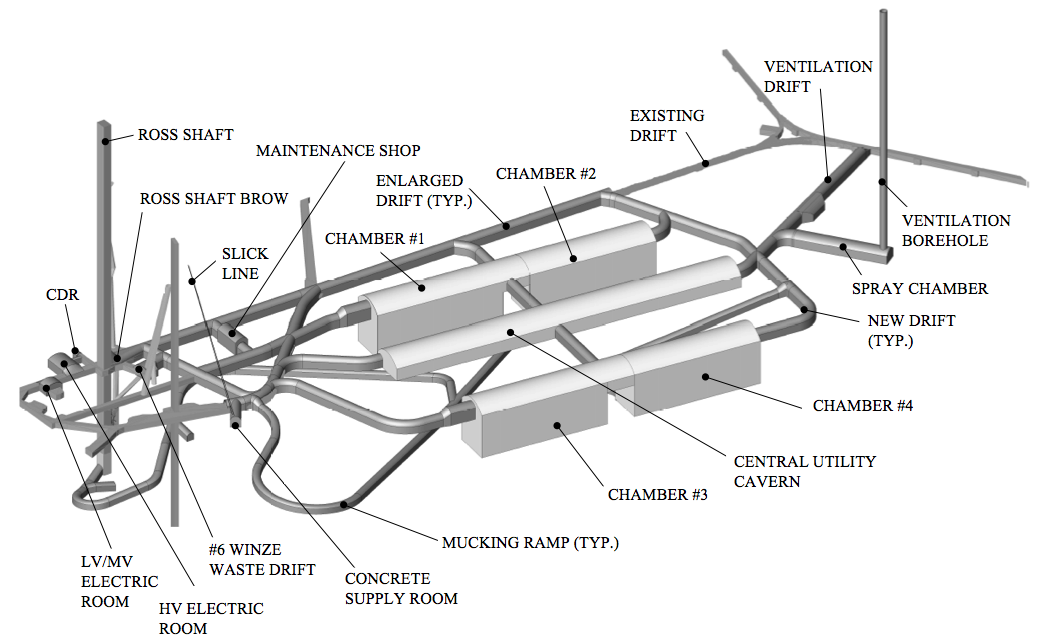
\includegraphics[width=0.9\textwidth]{spaces-4850}
\end{cdrfigure}

%%%%%%%%%%%%%%%%%%%%%%%%%%%%%%%%%%%%%%%%%%%%%%%%%%%%%%%%%%%%%%%%%%%
\section{LBNF Caverns} %Cavities}
\label{sec:fscf-excav-cav}

%%%%%%%%%%%%%%%%%%%%%%%%%%%%%%%%%%
\subsection{Detector Caverns} %Cavities}
\label{sec:fscf-excav-det}

%\fixme{Almost everywhere we use `cavern' not `cavity'; am trying to make it consistent}

%The required underground spaces were defined through interaction with the DUNE design team such that they will accommodate the detector, utilities and cryogenics equipment required for DUNE to reach its scientific goals. 
The requirements from the Cryogenic Infrastructure and Far Detector subprojects on the caverns are mainly related to the dimensions of the space, and are documented in~\cite{dune-sci-req}.  The overall dimensions of the main caverns are shown in Figure~\ref{fig:dim-cavern-excav}. The DUNE detector modules will be housed in four chambers within two main caverns at the 4850L. 
%\fixme{tmoved into chap 1. Here it feels like `too little too late'} Siting deep underground is required to shield from cosmic rays, as detailed in Report on the Depth Requirements for a Massive Detector at Homestake [15]. The 4850L is deeper than what is absolutely required, but is used because of existing access at this level. 

\begin{cdrfigure}[Dimensions of the main LBNF cavern excavations]{dim-cavern-excav}{Dimensions of the main LBNF cavern excavations (final dimensions will be slightly smaller). (SURF) }
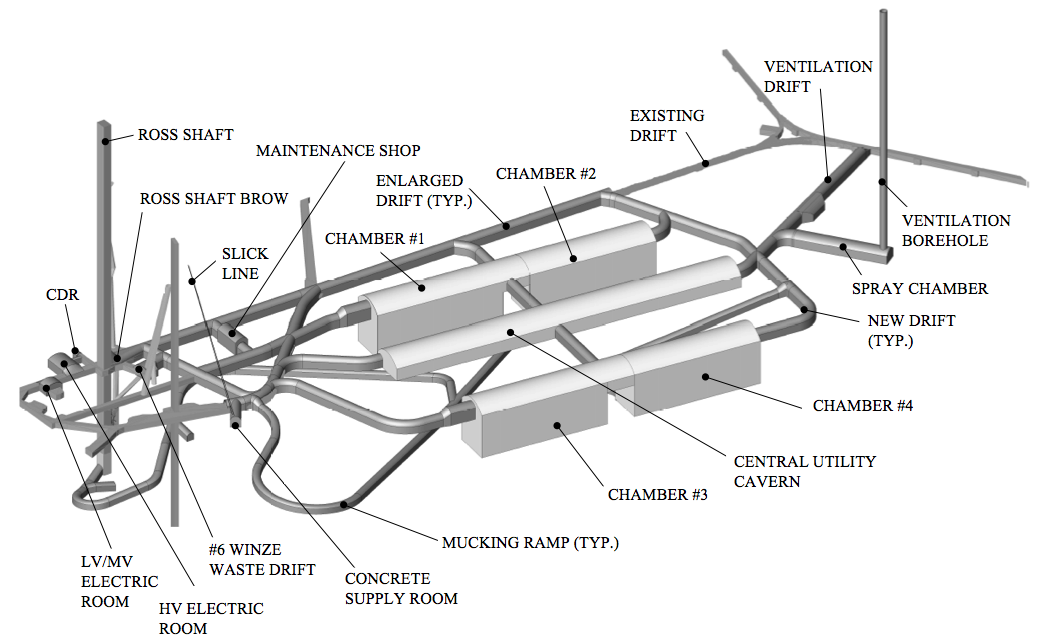
\includegraphics[width=\textwidth]{dim-cavern-excav} 
\end{cdrfigure}

The size %limit on size 
of a detector module is limited by both rock strength and the maximum dimensions of %limits on the ability to produce large dimension 
anode and cathode plane arrays that can be produced, lowered through the shaft and installed. Space occupied by the free-standing steel structure, the vessel's insulating liner, and an intentional exclusion zone reduce the total volume of the detector to less than the volume of the excavation; the fiducial volume is consequently reduced, as well. 
Current assessment of rock quality  for this formation indicates that caverns of the sizes indicated in Figure~\ref{fig:dim-cavern-excav} are reasonable. % with the rock quality assumed for this formation.

Preliminary modeling in both 2D and 3D of the proposed excavations has been done. % included 2D and 3D numerical modeling. 
The 2D models indicated that the intact rock strength and joint strength have the greatest impact on the design 
%The intact rock strength and joint strength had the greatest impact according to the 2D modeling, 
and the 3D results confirmed that the complex geometry of the design, that includes multiple drifts and caverns, is possible. 

The far detector %cavity 
caverns and drifts will be supported using galvanized rock bolts/cables, wire mesh, and fiber-reinforced shotcrete to allow a lifetime of 30 years. The floor of the cavern %cavity 
has been evaluated and does not require support. \fixme{how do you know if they're not excavated yet? And are we talking about all the caverns, or a specific one?} 

Groundwater is another factor to consider when planning the excavations. All experience, analysis, and field testing at the 4850L of SURF indicate that the volume of water to be encountered will be very minor ($\ll$1~lpm),  but that the locations of these small seeps are unpredictable. %To accommodate whatever water is encountered, 
A groundwater drainage system will be placed behind the shotcrete in the arch and walls of the far detector cavern rock excavation to collect %. This drainage system will collect groundwater (native) 
the seepage and eliminate the potential for hydrostatic pressure build-up behind the shotcrete. Channels will be placed in the concrete invert to drain groundwater to the sump system. 


%%%%%%%%%%%%%%%%%%%%%%%%%%%%%%%%%%  
\subsection{Structure and Cranes}
\label{sec:fscf-excav-cranes}

The LBNF caverns require monorail cranes to facilitate the construction of the cryostats and detector components. Placement of rock bolts will be coordinated with the excavation contractor to provide anchorage to support these monorails.

%%%%%%%%%%%%%%%%%%%%%%%%%%%%%%%%%%%%%%%%%%%%%%%%%%%%%%%%%%%%%%%%%%%
\section{LBNF Central Utility Cavern}
\label{sec:fscf-excav-util-cav}

LBNF requires space for cryogenics equipment outside the detector chambers. Space is also required for conventional facilities utilities. It is planned to excavate an independent central cavern, called  the Central Utility Cavern, to house the experiment's cryogenics systems, the electrical equipment to supply power for both facility and experiment needs, sump pump access and controls, fire sprinkler room, air handling units (AHUs), a chilled-water system and ducting. The centralized location minimizes overall utility distribution and the associated costs. Furthermore, isolating the utilities from the experiment simplifies electrical ground isolation, making it easier to avoid interference with sensitive detector electronics. Finally, it provides the opportunity to optimize ventilation; the heat emanating from the equipment can be controlled in this one cavern. 

%%%%%%%%%%%%%%%%%%%%%%%%%%%%%%%%%%%%%%%%%%%%%%%%%%%%%%%%%%%%%%%%%%%
\section{Access/Egress Drifts}
\label{sec:fscf-excav-access-drifts}

All the equipment that comes down the Ross Shaft must also pass through the drift connections to get to the new LBNF excavations. The drift therefore needs to accommodate not only the largest possible load from the shaft but also utilities installed in the drift itself. The drift connection sizes will be optimized accordingly. 
%In order to accommodate deliveries, the drift connections from the Ross Shaft to the new LBNF excavations will be optimized to accommodate the maximum load size possible through the shaft plus the utilities required to service the facility. 
At the writing of this document, an assumed size of 5~m wide by 6~m tall is used for all access and egress drifts. All new excavations, or drifts enlarged for LBNF will be provided with a shotcrete wall (rib) and ceiling (back) and a concrete floor (sill).

%%%%%%%%%%%%%%%%%%%%%%%%%%%%%%%%%%%%%%%%%%%%%%%%%%%%%%%%%%%%%%%%%%%
\section{Excavation Sequencing}
\label{sec:fscf-excav-exc-seq}

A key goal of LBNF and DUNE is to complete construction and start operation of the first 10-kt detector as early as possible. To %facilitate 
this end, the excavation will be sequenced such that LBNF can begin installation of a cryostat in the first detector chamber while excavation continues into the second chamber in the same cavern.  A temporary wall will be built in the detector installation laydown space (this is the area between detector chambers that is not as deep as the chambers themselves, sometimes called the `'rock pillar'') to isolate one  from the other. 
This wall must be %of sturdy construction
sturdy enough to withstand the air shock waves associated with drill-and-blast type %construction. 
excavation.  % Further evaluation of 
Vibration limits and controls must be further evaluated %considered 
as the design advances to avoid damaging the cryostat as it is assembled next-door to the excavation of the second chamber.

In addition to controlling the impacts from blasting, logistical coordination is a key concern with a sequenced excavation schedule in which cryostat construction is concurrent with excavation. %Many experiment 
Cryostat and detector components will need to be delivered through the Ross Shaft, which will also be used for loads associated with excavation and other construction activities. A logistics study\cite{lbnf-logistics} has been performed to evaluate whether this can be done without impact on either civil or experiment construction.  This study confirmed that with good coordination (led by the construction manager) this single shaft can support all anticipated material and personnel transport. %deliveries.  
The Yates shaft can provide some relief during high-intensity work periods, but this was not factored into %considered 
in the study; therefore the results are conservative. % to evaluate the most conservative approach.

Most excavated material will travel through a mucking ramp starting at the base of each detector chamber and ending at the waste dump near the Ross Shaft, as illustrated in Figure~\ref{fig:spaces-4850}. This %route 
ramp is completely independent of all other traffic and is outfitted with %includes 
a separate ventilation stream to keep diesel exhaust from %other 
the occupied spaces. During times when excavation is establishing the upper sections of the caverns and developing a means of dumping excavated material to this lower elevation, material will need to be transported at the 4850L. \fixme{What drawing can we reference?}
 To alleviate any potential interferences, the first phase of construction will establish a connection from the 4850L to the mucking ramp \fixme{`from the 4850L' in a detector chamber? what level is the ramp at?  Josh} , as well as ventilation paths to avoid contaminating the air in spaces that have been turned over for cryostat construction. 

Delivery of cryostat components to the individual chambers can be accomplished in one of two ways. 
\fixme{Instead can we say ``Delivery of cryostat components to the individual chambers can be made to  one of two areas''?} All materials are delivered through the shafts to the 4850L, which is $\sim$18m above the base of the chambers. During construction of the first cryostat, while excavation continues in the other areas, all materials will be delivered to the detector installation laydown area between the first and second detector chambers and/or to the west end of the first detector chamber. An overhead crane will be used to lower this material into the chambers. Excavation in chambers 3 and 4 will be accomplished in parallel and will be complete before cryostat construction begins. %This leaves open the option of using the mucking ramp for delivery of cryostat components \fixme{for modules 3 nd 4?}. This ramp has been designed at an 8\% grade to from \fixme{to or from?} the west side to allow for this possibility. 

%%%%%%%%%%%%%%%%%%%%%%%%%%%%%%%%%%%%%%%%%%%%%%%%%%%%%%%%%%%%%%%%%%%
\section{Interfaces between DUNE, Existing Facilities, Cryogenics and Excavation}
\label{sec:fscf-excav-interfaces}

There are several points at which the experiment and the facility interface closely. These are coordinated between the design teams for DUNE, LBNF Cryogenics Infrastructure and LBNF Conventional Facilities, and design consultants. Sizing of spaces and components, and sequencing of construction figure among the key issues, listed here, that interfaces must address.
\begin{itemize}
\item The LBNF cryostats are freestanding structures requiring infrequent 
access for inspection around the structures' perimeters. %\fixme{I removed `infrequent' because it removed the focus from the space issue and made it sound less important}
\item The utility spaces to house the equipment for the cryogenics system are directly influenced by the size of the equipment.
\item The size and construction sequencing of the detector chambers are critical to the DUNE experiment strategy.
\end{itemize}

In addition to these interfaces, the LBNF excavation requires coordination with existing facilities and activities, in particular, with experiments located in relatively close ($\sim$100~m) proximity to the planned excavation.  %To manage the risks associated with 
A test blast program has been designed to study the actual response of the rock mass in this area due to vibrations and air-blast overpressure created by drill-and-blast excavation techniques.  This test blast program is currently being coordinated closely with the existing experiments % as of the writing of this report, 
and the %actual physical 
test itself %is planned to 
will be completed within the first quarter of FY16.  The results of this test will %should 
either confirm that the planned excavation approach is appropriate, or indicate where %define 
modifications to the plan must be made. %that may be necessary in the areas closest to the existing facilities.





